\section{A description of \acs{EsPy}}

\subsection{Why \textsc{Python}?}
There a number of reasons why \textsc{Python} was the chosen programming
language for \ac{EsPy}, beyond the fact that the candidate had a decent
familiarity with it when starting their PhD:
\begin{itemize}
    \item It has a large user-base, particularly within the scientific
        community.
    \item The \textsc{SciPy} ecosystem\cite{Virtanen2020}, including the packages
        \textsc{NumPy}\cite{Harris2020} and
        \textsc{Matplotlib}\cite{Hunter2007} is a powerful tool which enables
        high-performance scientific computation in \textsc{Python}, despite the
        language's reputation for performing slowly.
    \item Being a scripting language makes \textsc{Python} ideal for
        exploring datasets in a step-by-step fashion. This is useful in the
        context of \ac{EsPy}, as a user will want to
        (i) inspect and pre-process then data,
        (ii) determine the regions they wish to estimate setup the estimation routine,
        (iii) output the estimation result.
        This can be achieved easily by ``hacking'' and re-running
        \textsc{Python} scripts or by using ``notebook'' environments, such as
        \textsc{Jupyter}.
    \item It is free and open-source, as opposed to well-known scientific
        computing platforms such as \textsc{Matlab}\textregistered\ and
        \textsc{Mathematica}.
    \item \textsc{Python} supports sophisticated object-oriented programming
        features, such as multiple levels of inheritance. This is exploited in
        \ac{EsPy} in order to create numerous objects designed with a specific
        \ac{NMR} data types in mind.
\end{itemize}

Probably the largest in using \textsc{Python} is its slow performance on
account of it being an interpreted, dynamically typed language with relies on
garbage collection for memory management. While \textsc{NumPy} provides
interfaces to run fast computations with pre-compiled C-code, a significant
performance benefit would likely be realised if a low-level compiled language
like C, C++, or \textsc{Rust} were used instead. While this may be so, the
development time in writing programs with these lower-level languages is
typically a lot greater than with a language with a higher level of abstraction
like \textsc{Python}.

\subsection{Estimator objects}
\begin{figure}
    \centering
    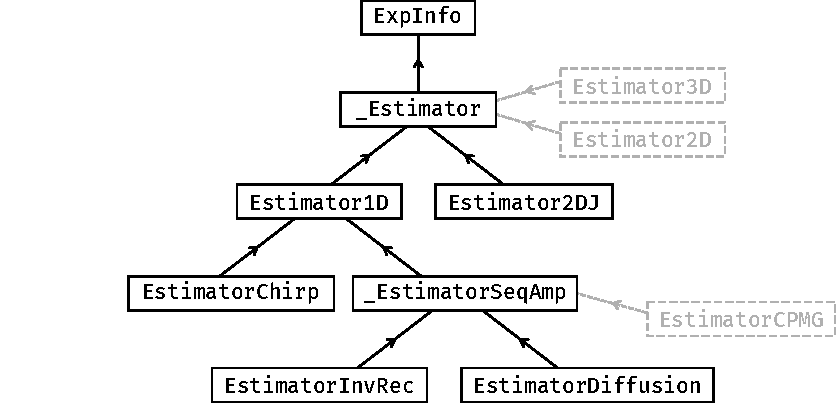
\includegraphics{inheritance_tree/inheritance_tree.pdf}
    \caption[
        Inheritance tree for estimation classes in the \acs{EsPy} package.
    ]{
        Inheritance tree for estimation classes in the \acs{EsPy} package.
        Arrows are directed from child classes to the parent class they
        directly inherit from. Classes in grey are objects that could be added
        to the \ac{API} in the future.
    }
    \label{fig:inheritance}
\end{figure}
The fundamental user-facing objects (or classes) that \ac{EsPy} provides are
\emph{estimators}.
Instances of these estimator objects contain relevant
\emph{attributes} (the \ac{FID}, experiment parameters like the sweep width,
transmitter offset etc), as well as \emph{methods} which perform useful
functions like estimation, figure generation etc.
Thanks to \textsc{Python}'s support for multiple levels of inheritance, it is
possible to build numerous objects with certain shared attributes and methods,
but that also have their own bespoke features that are solely of relevance to
the type of \ac{NMR} data being considered. Figure \ref{fig:inheritance} is an
inheritance diagram for the estimators in \ac{EsPy}.

\begin{itemize}[leftmargin=0pt,label={}]
    \item[] \textbf{\textbf{\texttt{ExpInfo}}}: Stores parameters used in a particular \ac{NMR}
        experiment. \texttt{ExpInfo} also has methods for the generation of the
        timepoints/chemical shifts sampled by the experiment, and for producing
        synthetic \acp{FID}, if given a set of oscillator parameters.
    \item[] \textbf{\texttt{\_Estimator}}: Also possesses the \ac{NMR} data as an
        attribute on top of the experiment information. This class is
        designed to contain the functionality which can be generalised across
        all \ac{NMR} data types considered. It does not however possess all the
        features necessary to useful as a standalone object, and as such the
        user is not permitted to use it directly (such an object is referred to
        as an \emph{abstract class}). For child classes of
        \texttt{\_Estimator}, the main feature that requires methods to be
        defined is the means by which the data is imported (experimental data)
        or generated (simulated data).
    \item[] \textbf{\texttt{Estimator1D}}: \ac{1D} datasets, such as those in
        Section \ref{sec:evaluation} are analysed using this class.
    \item[] \textbf{\texttt{Estimator2DJ}}: Estimation of \ac{2DJ} data is
        performed with this class. It also provides features to generate ure
        shift spectra using \ac{CUPID} (Chapter \ref{chap:cupid}).
    \item[] \textbf{\texttt{\_EstimatorSeqAmp}}: An abstract class
        which enables the estimation of sequential \ac{1D} datasets as outlined
        in Section \ref{sec:seq}. Analysis of the dataset varies depending on
        the type of experiment considered, such as the function used for
        fitting amplitudes (Table \ref{tab:seq-equations}), and the means by
        which that data should be imported/generated. As such, this is not
        designed for direct use. One of the classes which inherit it should be
        used instead.
    \item[] \textbf{\texttt{EstimatorInvRec}}: For the estimation of inversion
        recovery ($T_1$) datasets.
    \item[] \textbf{\texttt{EstimatorDiffusion}}: For the estimation of
        diffusion datasets.
\end{itemize}

Other estimator objects which are yet to be implemented, but are potential
future additions to the package are also depicted in Figure
\ref{fig:inheritance}. \texttt{Estimator2D} and \texttt{Estimator3D} would be
for the estimation of datasets comprising sets of \ac{2D} or \ac{3D} amplitude-
or phase-modulated \acp{FID}, respectively. A discussion of the feasibility of
implementing these is made in Section \ref{sec:future-work}.

\section{The \acs{EsPy} \acs{GUI}}
\begin{figure}
    \centering
    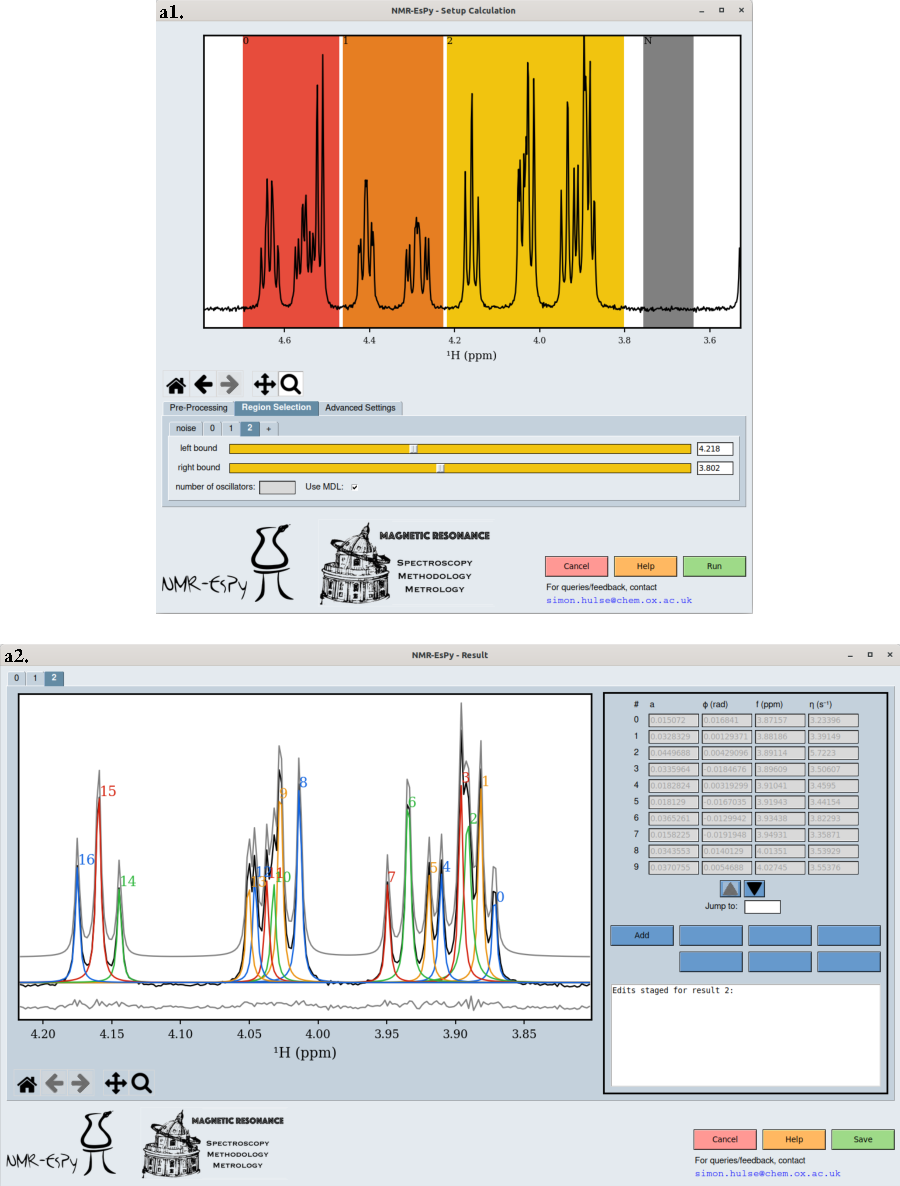
\includegraphics{gui/gui_1d.pdf}
    \caption[
        Screenshots of the \acs{EsPy} \acs{GUI} for \ac{1D} and \acs{2DJ} estimation.
    ]{
        Screenshots of windows that form part of the \ac{EsPy} \ac{GUI} for
        \ac{1D} estimation (\textbf{a.}) and \ac{2DJ} estimation (\textbf{b.}).
        For both data types, the windows used to setup the estimation routine
        (\textbf{1.}) and inspect the result (\textbf{2.}) are shown.
        (Continues on the next page)
    }
    \label{fig:gui}
\end{figure}
\begin{figure}%
    \ContinuedFloat
    \centering
    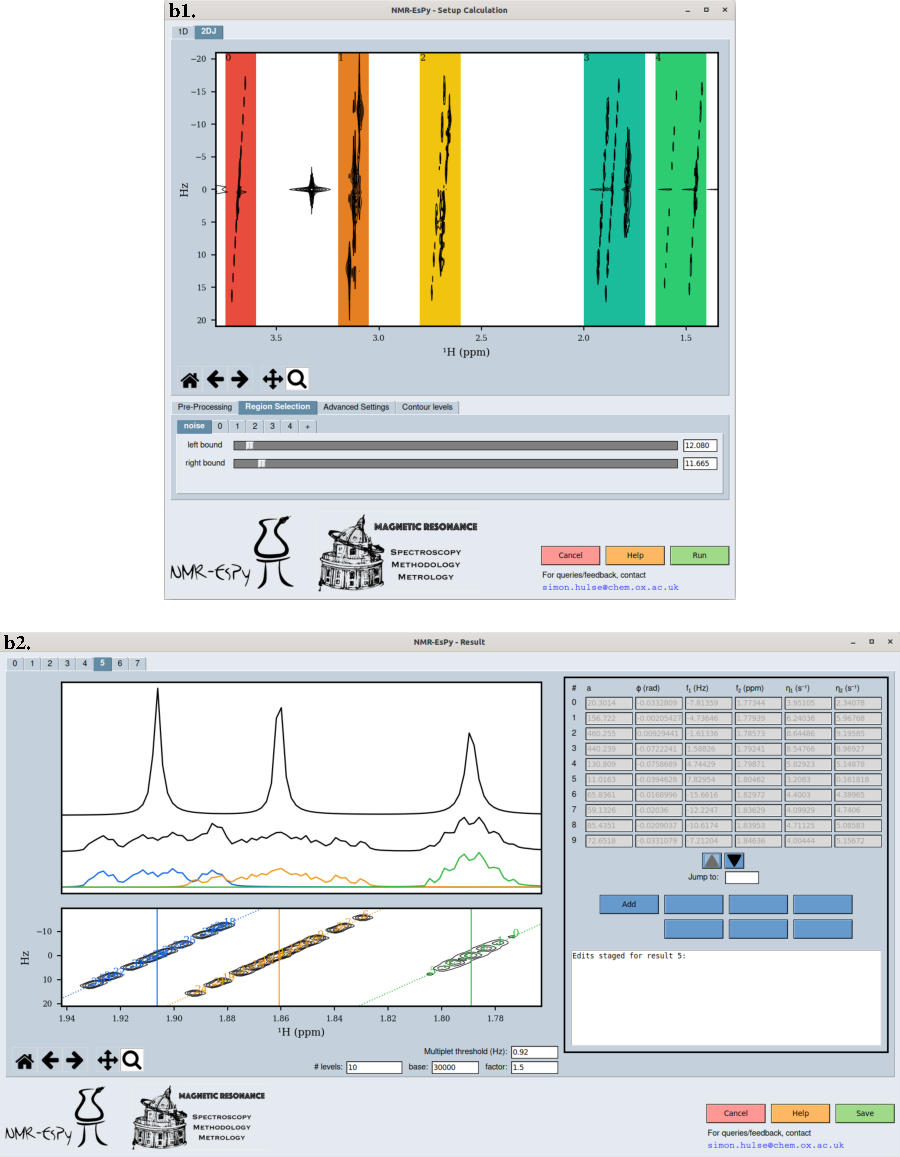
\includegraphics{gui/gui_2dj.pdf}
    \caption*{Continuation of \textbf{\textsc{Figure \ref{fig:gui}}}.}
\end{figure}
 Coloured rectangles in the plot indicate regions of the spectrum to generate
 frequency-filtered \acp{FID} from, the grey rectangle defines the noise
 region.
